\documentclass[12pt, french]{article}

\usepackage{fancyhdr, fancybox, lastpage}
\usepackage[most]{tcolorbox}
\usepackage[a4paper, margin={0.3in, .75in}]{geometry}
\usepackage{wrapfig}
\pagestyle{fancy}
\renewcommand\headrulewidth{1pt}
\renewcommand\footrulewidth{1pt}
\fancyhf{}
\rhead{ \em{Zakaria Haouzan}}
\lhead[C]{\em{1ére année baccalauréat Sciences Mathématiques}}
\chead[C]{}
\rfoot[C]{}
\lfoot[R]{}
\cfoot[]{\em{Page \thepage / \pageref{LastPage}}}


\newtcolorbox{Box2}[2][]{
                lower separated=false,
                colback=white,
colframe=white!20!black,fonttitle=\bfseries,
colbacktitle=white!30!gray,
coltitle=black,
enhanced,
attach boxed title to top left={yshift=-0.1in,xshift=0.15in},
title=#2,#1}


\begin{document}
\begin{center}
   \shadowbox {\bf{Energie potentielle d'une charge électrique dans un champ électrique uniforme }}
\end{center}


%%_________________________Exercice ! :"_________________________Exercice
   \begin{Box2}{Exercice 1 : }
Deux armatures métalliques $P_A$ et $P_B$, parallèles entre elles et distantes de d, sont reliées aux bornes d'un
générateur de tension continue. Entre ces deux armatures règne un champ électrostatique $\vec{E}$ uniforme.

1. Donner l'expression du travail de la force électrostatique $\vec{F}$ qui s'exerce sur une particule de charge q se
déplaçant d'un point A de l'armature $P_A$ à un point B de l'armature $P_B$. L'exprimer en fonction de E, AB et q.

      2. Montrer que le travail de cette force s'écrit : $W_{AB}(\vec{F})) = q.U_{AB}$.

      3.Calculer sa valeur dans le cas d'un noyau d'hélium $He^{2+}$ se déplaçant de A à B.

      Données : $e = 1,60 . 10^{-19}C; U_{AB}= 400 V$
   \end{Box2}


%%_________________________Exercice !2 :"_________________________Exercice
\begin{Box2}{Exercice 2 : }
\begin{wrapfigure}{r}{0.28\textwidth}
  \begin{center}
    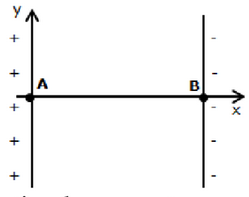
\includegraphics[width=0.28\textwidth]{./img/img_00.png}
  \end{center}
\end{wrapfigure}




Une particule $\alpha$(noyau d'hélium), produite par une source radioactive, est émise au voisinage d'un point A. La
valeur de sa vitesse en A est négligeable devant celle qu'elle peut atteindre en B.
Entre les points A et B règne un champ électrostatique uniforme qui permet l'accélération de la particule. Le poids et les frottements sont négligeables lors de ce mouvement.

   1. Quelle est la charge $q_\alpha$ de la particule $\alpha$?

   2. Établir l'expression du travail de la force électrostatique s'appliquant sur la
particule $\alpha$ se déplaçant entre A et B. Exprimer ce travail en fonction $q_\alpha$, $V_A$ et $V_B$.
($V_A$ et $V_B$ sont les potentiels respectifs aux points A et B.)

3. En déduire l'expression de la variation d'énergie potentielle électrique entre A et B.

 4. L'énergie mécanique se conserve-elle? Justifier.

5. À partir des réponses précédentes, exprimer la différence de potentiel $V_A - V_B$ en fonction de $v_B$, $m_\alpha$ et $q_\alpha$.
   et calculer cette valeur sachant que la vitesse en B a pour valeur $v_B = 1,00 . 10^3 km.s^{-1}$
.

   Données : $e = 1,60 . 10^{-19} C; m_\alpha= 6,70 . 10^{-27} kg$.
\end{Box2}

%%_________________________Exercice ! 3:"_________________________Exercice
\begin{Box2}{Exercice 3 :}
\begin{wrapfigure}{r}{0.28\textwidth}
  \begin{center}
    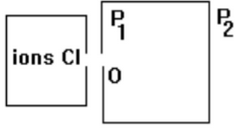
\includegraphics[width=0.28\textwidth]{./img/img_01.png}
  \end{center}
\end{wrapfigure}


   Par l’ouverture O deux ions $^{37}_{17}Cl^-$ et $^35Cl^-$
(isotopes de l’élément chlore) pénètrent avec une vitesse pratiquement nulle dans une région située entre deux plaques $P_1$ et $P_2$ où règne un champ électrostatique uniforme $\vec{E}$

   1. Si $(V_{P2} - V_{P1})$ est égale à 100 V, quelle est en eV l’énergie acquise par chaque
ion à l’arrivée en $P_2$ ?

   2. En déduire le rapport des vitesses des ions à leur arrivée en $P_2$.

   Données: - masse molaire de l’ion $^{35}Cl^- : 35.10^{-3}$ kg/mol ;

   - masse molaire de l’ion $^{37}Cl^-$:$37.10^{-3}$kg/mol ;

   - Constante d’Avogadro:$N = 6,02.10^{23} mol^{-1}$ .
\end{Box2}
\vspace{3cm}
\begin{center}
   \Large{ \em{Exercices Supplémentaires}}
\end{center}


%%_________________________Exercice 4 : _________________________Exercice
\begin{Box2}{Exercice 4 : }
Deux plaques métalliques carrées de cote l, sont placées en regard, parallèlement l’une à l’autre
dans une enceinte où règne un vide poussé. En chargeant les plaques, on crée entre elles un
champ électrique uniforme de vecteur E . Un faisceau des électrons pénètre en O dans la région
du champ et en sort en S. le poids des électrons a un effet négligeable sur leur mouvement. Les
figures 1 à 4 donnent la trajectoire des électrons dans quatre cas. (voir les figures )
  \begin{center}
    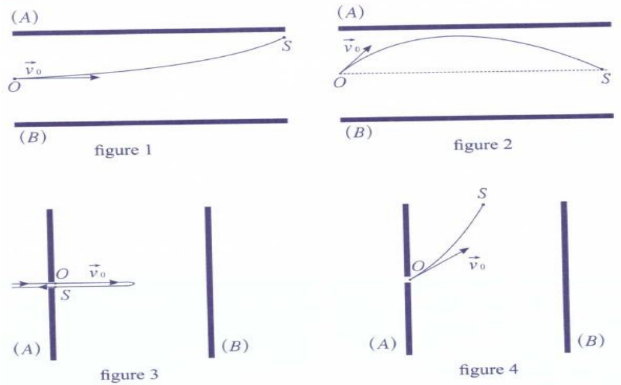
\includegraphics[width=0.8\textwidth]{./img/img_02.png}
  \end{center}
   1. Dans chacun des cas, indiquer la direction et le sens du vecteur champ E et préciser le
   signe de la tension $U_{AB}$.

   2. A partir du théorème de l’énergie cinétique, montrer que la variation d’énergie cinétique
entre O et S ne dépend que de e, E et OS . 

   3. Préciser dans chaque expérience si l’énergie cinétique augmente, diminue ou reste
constante entre O et S.

   4. Les électrons pénètrent avec une vitesse $v_o = 6. 10^5m/s$, entre les plaques de déviation
verticale, en un point O situé à égale distance de chacune d’elles. Lorsque la tension $U=500V$ est appliquée à ces plaques distantes de d = 10cm, les électrons sortent de l’espace

champ en un point S tel que OS = d’ = 2cm. (figure 1)
   \begin{enumerate}
      \item[a.] On prend l’origine des potentiels $V_o = 0$ au point O. Calculer Vs potentiel électrostatique du
point S de l’espace champ. 
\item[b.] Déterminer Epo et Eps, énergies potentielles électrostatique d’un électron en O et en S dans
l’espace champ, en joules et en électronvolts.
         \item[c.] En déduire Ecs énergie cinétique de sortie des électrons, en électronvolts.
   \end{enumerate}
\end{Box2}


%%_________________________Exercice 5 : _________________________Exercice
%\begin{Box2}{Exercice 5 : }

%\end{Box2}
%%%_________________________Exercice 6 : _________________________Exercice
\end{document}
